%!TEX root = main.tex
\section{Non-Linear Models}

In this section, we extend our framework to approximate arbitrary classification losses within arbitrarily small bias. 
Although theoretically justified, this framework can become heavyweight for loss functions which are not well approximable by polynomials 
(e.g., hinge). We provide efficient quantization heuristics for these loss functions. 

\subsection{Quantizing Arbitrary Polynomials} 

Assume we are given a degree $d$ polynomial $P(x) = \sum_{i = 0}^{d} m_i z^i$, and that 
we wish to evaluate it at $\vec{a}^\top \vec{x}$, while quantizing $\vec{a}$, so as to preserve the value of $P( \vec{a}^\top \vec{x})$ in expectation. 
We do so as follows. 

We will use $d$ independent quantizations of $\vec{a}$, $Q_1(\vec{a}), Q_2(\vec{a}), \ldots, Q_d(\vec{a})$. 
Given these quantizations, our reconstruction of the polynomial will be 
$$ Q(P) := \sum_{i = 0}^d m_i \prod_{j \leq i} Q_j(\vec{a})^\top \vec{x}.$$

The fact that this is an unbiased estimator of $P( \vec{a}^\top \vec{x} )$ follows from the independence of the quantizations. Extending the analysis in Lemma~\ref{lem:qbound} yields:

\begin{lemma}
\label{lem:poly-sec-moment-bound}
	$\E[ Q(P)^2 ] \leq 2^d \sum_{i = 0}^d m_i r(s)^i (\vec{a}^\top \vec{x})^i.$
\end{lemma} 








\subsection{Quantizing Arbitrary Classification Losses}

Assume a standard classification setting, where we have samples $[(\vec{a}_i, b_i)]_i$ drawn from a distribution $\mathcal{D}$, a loss function $\ell: \R \rightarrow \R$, and we wish to find $\vec{x}$ which minimizes $\E_{\mathcal{D}} [ \ell( b \cdot \vec{a}^\top \vec{x} ]$. The gradient of $\ell$ is given by 
$$ \nabla_\vec{x} (b \cdot \vec{a}^\top \vec{x}) = b \ell' (b \cdot \vec{a}^\top \vec{x}) \vec{a}.$$

Assume normalized samples, i.e. $\| \vec{a}_i \|_2 \leq 1, \forall i$, and that $\vec{x}$ is constrained such that $\| \vec{x} \|_2 \leq R$, for some real value $R > 0$. We are given a target accuracy $\epsilon$, within which we wish to approximate the gradient. 

Given this, we fix the minimal-degree polynomial $P$ such that $|P(z) - \ell'(z)| \leq \epsilon, \forall z \leq R$. This polynomial is known to both transmitter (sample source) and receiver (compute device). The protocol is as follows. 
\begin{itemize}
	\item For a given sample $(\vec{a}_i, b_i)$ to be quantized, the source will transmit $b_i$, as well as $d + 1$ independent quantizations $Q_1, Q_2, \ldots, Q_{d + 1}$ of $\vec{a}_i$. 
	\item The receiver computes $b \cdot Q(P) Q_{d + 1} ( \vec{a}_i )$ and uses it as the gradient.
\end{itemize}

It is easy to see that the bias in each step is bounded by $\epsilon$. 
We can extend Lemma~\ref{lem:poly-sec-moment-bound} to obtain a general bound on convergence. 

\begin{lemma}
	\textcolor{red}{DAN: TODO here}
\end{lemma}

\paragraph{Chebyshev Approximations} 
For \emph{hinge loss}, the gradient is the step function, which is hard to approximate generally by polynomials. 
However, the problem is well studied for intervals of the type  $[-R, R] \setminus [-\delta, \delta]$, for some small parameter $\delta > 0$~\cite{frostig2016principal, allen2016faster}; the latter reference provides the optimal approximation via Chebyshev polynomials, which we use in our experiments. 

For \emph{logistic loss}, with sigmoid gradient, we again notice that polynomial approximations have been well studied. In particular, we use the optimal Chebyshev polynomial approximation of~\cite{vlcek2012chebyshev}. 

Figure~\ref{fig:approximation} shows how close the Chebyshev polynomial aprroximations with different degrees are to those two kind of functions.
\begin{figure}[h]
\centering
    \begin{subfigure}[h]{.4\columnwidth}
    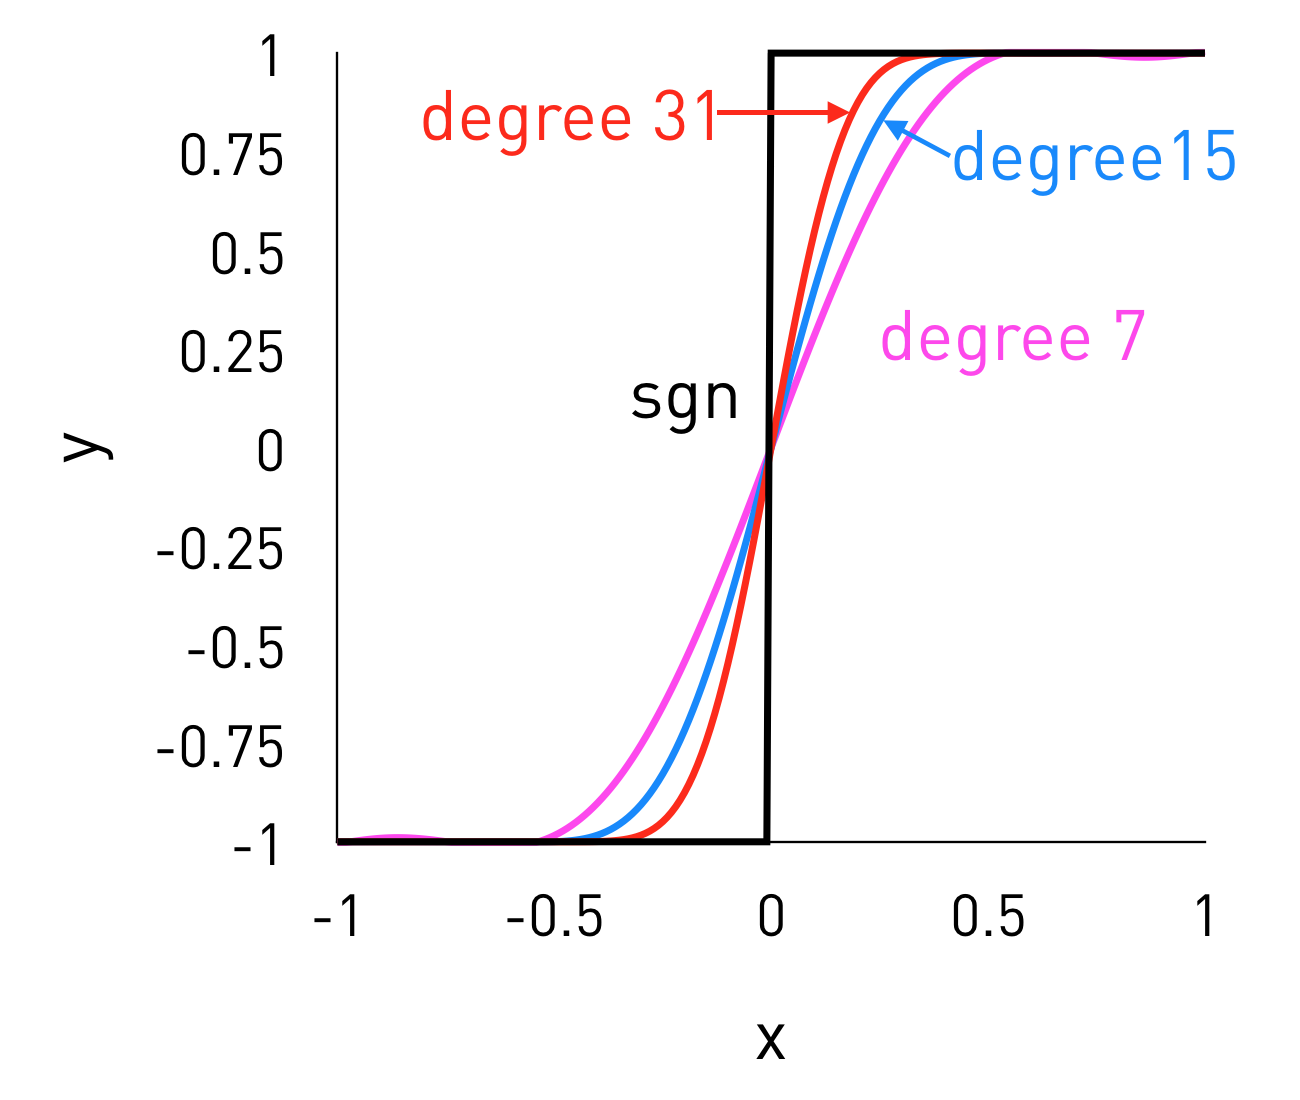
\includegraphics[width=\columnwidth]{micro-experiments/chebyshev_sgn} 
    \caption{sign function}
    \end{subfigure}
    \begin{subfigure}[h]{.4\columnwidth}
    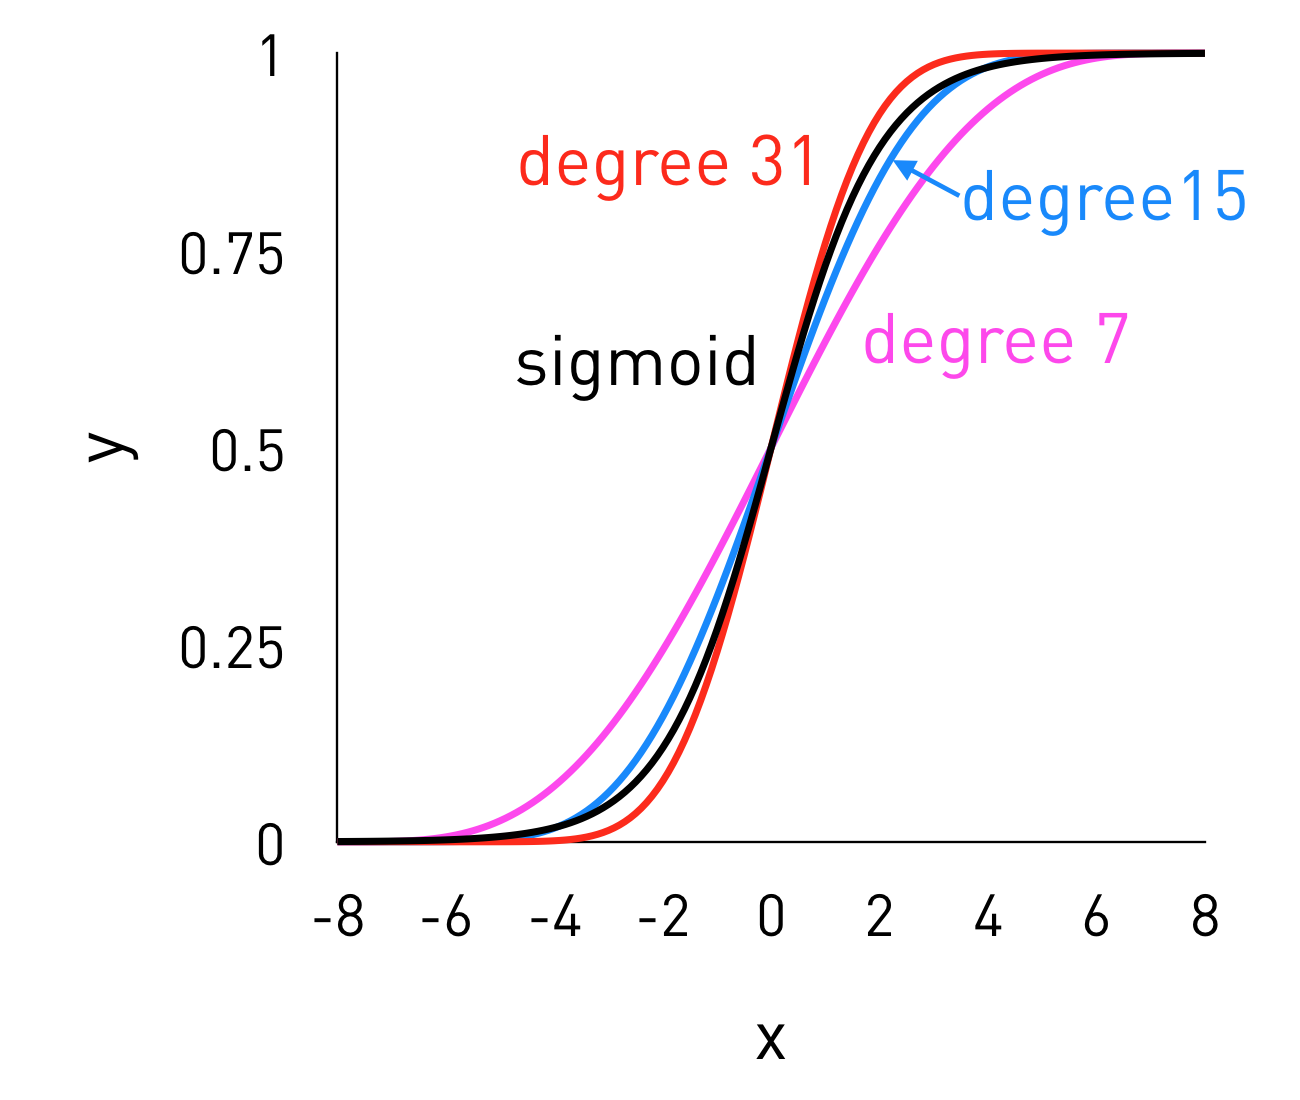
\includegraphics[width=\columnwidth]{micro-experiments/chebyshev_sigmoid} 
    \caption{sigmoid function}
    \end{subfigure}
\caption{Chebyshev approximation to gradient of hinge loss and logistic loss with different degrees}
\label{fig:approximation}
\end{figure} 

\paragraph{Practical Considerations} The above strategy introduces a precision-variance trade-off, since increasing the precision of approximation (higher polynomial degree) also increases the variance of the gradient. 
Fortunately, we can further reduce the variance and increase the approximation quality by increasing the density of the quantization. 
The results in Section~\ref{sec:exp} show that a total of $8$ bits per sample is sufficient to ensure convergence to the same result as the full-precision 
implementation for both hinge loss and logistic loss. 


